% ============================================================
% Template LaTeX ABNT NBR 14724/2024 — IFB
% ============================================================

\documentclass[
  12pt,
  a4paper,
  oneside,
  brazil,
  chapter=TITLE
]{article}

\usepackage[T1]{fontenc}
\usepackage[utf8]{inputenc}
\usepackage[brazil]{babel}
\usepackage{mathptmx}

\usepackage[
  a4paper,
  left=3cm,
  top=3cm,
  right=2cm,
  bottom=2cm,
  headheight=14pt,
  headsep=0.5cm
]{geometry}

\usepackage{setspace}
\onehalfspacing

\usepackage{indentfirst}
\setlength{\parindent}{1.25cm}
\setlength{\parskip}{0pt}

\usepackage{titlesec}

\titleformat{\section}
  {\normalfont\normalsize\bfseries\MakeUppercase}
  {\thesection\quad}
  {0em}{}

\titleformat{\subsection}
  {\normalfont\normalsize\bfseries}
  {\thesubsection\quad}
  {0em}{}

\titleformat{\subsubsection}
  {\normalfont\normalsize\bfseries\itshape}
  {\thesubsubsection\quad}
  {0em}{}

\titlespacing*{\section}      {0pt}{18pt}{12pt}
\titlespacing*{\subsection}   {0pt}{18pt}{6pt}
\titlespacing*{\subsubsection}{0pt}{12pt}{6pt}

\newcommand{\secbreak}{\clearpage}
\let\oldsection\section
\renewcommand{\section}{\secbreak\oldsection}

\usepackage{fancyhdr}
\pagestyle{fancy}
\fancyhf{}
\fancyhead[R]{\fontsize{10}{12}\selectfont\thepage}
\renewcommand{\headrulewidth}{0pt}
\renewcommand{\footrulewidth}{0pt}

\fancypagestyle{plain}{
  \fancyhf{}
  \fancyhead[R]{\fontsize{10}{12}\selectfont\thepage}
  \renewcommand{\headrulewidth}{0pt}
}

\usepackage{longtable}
\usepackage{booktabs}
\usepackage{array}
\usepackage{multirow}
\usepackage{tabularx}
\renewcommand{\arraystretch}{1.3}

\usepackage{caption}
\DeclareCaptionFormat{abnt}{\fontsize{10}{12}\selectfont#1#2#3}
\DeclareCaptionLabelSeparator{emdash}{ --- }
\captionsetup{
  format=abnt,
  justification=centering,
  singlelinecheck=false,
  labelsep=emdash,
  position=above,
  skip=3pt
}

\newcommand{\fonte}[1]{%
  \begin{flushleft}
    \fontsize{10}{12}\selectfont Fonte: #1
  \end{flushleft}
}

\usepackage{enumitem}
\setlist{nosep, leftmargin=*}

\usepackage{tocloft}
\renewcommand{\contentsname}{SUMÁRIO}

\newlistof{quadros}{loq}{LISTA DE QUADROS}
\setlength{\cftquadrosindent}{0pt}
\setlength{\cftquadrosnumwidth}{0pt}
\makeatletter
\renewcommand{\listofquadros}{%
  \section*{LISTA DE QUADROS}%
  \@starttoc{loq}%
}
\makeatother

\newcommand{\quadrotitle}[2]{%
  \vspace{1em}%
  \phantomsection\label{quadro#1}%
  \addcontentsline{loq}{quadros}{Quadro #1 --- #2}%
  \noindent\textbf{Quadro #1 --- #2}\par\vspace{0.3em}%
}
\newcommand{\quadrofonte}[1]{\par\noindent\textit{Fonte: #1}\vspace{1em}\par}

\PassOptionsToPackage{hyphens}{url}
\usepackage[hidelinks, colorlinks=false, breaklinks=true]{hyperref}

\usepackage{quoting}
\quotingsetup{font=small, indentfirst=false, vskip=\baselineskip}

\usepackage[normalem]{ulem}
\usepackage{graphicx}
\usepackage{float}

\usepackage[
  alf,
  abnt-emphasize=bf,
  abnt-etal-cite=2,
  abnt-etal-list=0
]{abntex2cite}

\date{}

\begin{document}

% ══════════════════════════════════════════════════════════════════════════════
% CAPA
% ══════════════════════════════════════════════════════════════════════════════
\begin{titlepage}
  \thispagestyle{empty}
  \begin{center}

    \vspace{2cm}

    {\normalsize\bfseries
      INSTITUTO FEDERAL DE EDUCAÇÃO, CIÊNCIA E TECNOLOGIA DE BRASÍLIA\\[0.3em]
      \textit{Campus} Samambaia\\[0.3em]
      Curso Superior de Tecnologia em Design de Produto
    }

    \vfill

    {\large\bfseries
      PROCESSOS DE BENEFICIAMENTO DO AÇO E IMPLICAÇÕES PARA O DESIGN DE PRODUTO: RELATÓRIO DE VISITA TÉCNICA À GRAVIA INDÚSTRIA DE PERFILADOS DE AÇO
    }

    \vfill

    {\normalsize Brasília/DF\\2026}

  \end{center}
\end{titlepage}
\setcounter{page}{2}

% ══════════════════════════════════════════════════════════════════════════════
% FOLHA DE ROSTO
% ══════════════════════════════════════════════════════════════════════════════
\begin{titlepage}
  \thispagestyle{empty}
  \begin{center}

    {\normalsize\bfseries VICTOR HUGO DA SILVA COSTA}

    \vfill

    {\large\bfseries PROCESSOS DE BENEFICIAMENTO DO AÇO E IMPLICAÇÕES PARA O DESIGN DE PRODUTO: RELATÓRIO DE VISITA TÉCNICA À GRAVIA INDÚSTRIA DE PERFILADOS DE AÇO}

    \vfill

    \begin{flushright}
      \begin{minipage}{0.5\textwidth}
        \normalsize
        Relatório de Visita Técnica apresentado ao Curso Superior de Tecnologia em Design de Produto do Instituto Federal de Educação, Ciência e Tecnologia de Brasília, \textit{Campus} Samambaia, como requisito parcial para a aprovação na disciplina de Materiais e Processos de Fabricação I.

        \vspace{1em}
        Prof.ª Keila Sanches
      \end{minipage}
    \end{flushright}

    \vfill

    {\normalsize Brasília/DF -- 2026}

  \end{center}
\end{titlepage}

% ══════════════════════════════════════════════════════════════════════════════
% RESUMO
% ══════════════════════════════════════════════════════════════════════════════
\clearpage
\thispagestyle{empty}
\begin{center}
  {\normalsize\bfseries RESUMO}
\end{center}

\vspace{1em}
\noindent
Este relatório registra a visita técnica realizada em 02 de junho de 2026 à Gravia Indústria de Perfilados de Aço, em Taguatinga, Distrito Federal, e analisa os processos observados sob a perspectiva do design de produto. A planta industrial é organizada em galpões especializados: o Galpão 1 concentra operações de corte e conformação de chapas; o Galpão 3 é dedicado à perfilação contínua para drywall; e os Galpões 4, 5 e 6 atendem ao processamento de chapas espessas. Os principais processos identificados (corte a laser, corte a plasma, conformação por dobra em prensas hidráulicas e perfilação contínua) são descritos com base na observação direta e analisados em termos de capacidades, limites e relevância para decisões projetuais. O relatório argumenta que a compreensão dos processos de fabricação disponíveis é condição para que o designer especifique materiais e formas com realismo técnico.

\vspace{1em}
\noindent\textbf{Palavras-chave:} Beneficiamento do aço; Processos de fabricação; Design de produto; Corte a laser; Conformação por dobra.

% ══════════════════════════════════════════════════════════════════════════════
% LISTA DE FIGURAS
% ══════════════════════════════════════════════════════════════════════════════
\clearpage
\thispagestyle{empty}
\renewcommand{\listfigurename}{LISTA DE FIGURAS}
\listoffigures

% ══════════════════════════════════════════════════════════════════════════════
% LISTA DE QUADROS
% ══════════════════════════════════════════════════════════════════════════════
\clearpage
\thispagestyle{empty}
\listofquadros

% ══════════════════════════════════════════════════════════════════════════════
% SUMÁRIO
% ══════════════════════════════════════════════════════════════════════════════
\clearpage
\thispagestyle{empty}
\tableofcontents

% ══════════════════════════════════════════════════════════════════════════════
% CORPO DO TEXTO
% ══════════════════════════════════════════════════════════════════════════════

\section{Introdução}

Existe uma distância habitual entre o desenho e a fábrica. O designer projeta formas; o fabricante enfrenta chapas, prensas e tolerâncias. Enquanto essa distância não é percorrida de forma concreta, os projetos tendem a oscilar entre dois extremos igualmente problemáticos: o excesso de autocensura diante de processos que se imagina mais limitantes do que são, e a especificação de geometrias cuja viabilidade fabril nunca foi verificada.

A visita técnica à unidade industrial da Gravia Indústria de Perfilados de Aço, realizada em 02 de junho de 2026, funcionou como travessia deliberada dessa distância. A Gravia opera há mais de seis décadas na transformação e beneficiamento do aço para os setores da construção civil, indústria e agronegócio, com planta instalada em Taguatinga, Distrito Federal. O objetivo da visita foi observar os processos de beneficiamento em operação, compreender a organização produtiva e, principalmente, perceber o que cada processo comunica ao designer de produto em termos de liberdades e restrições projetuais.

Este relatório organiza os processos observados, descreve seus parâmetros e articula, ao final, as implicações que carregam para a prática do projeto.

\section{A empresa e a organização da produção}

A planta da Gravia é dividida em galpões com funções especializadas, o que permite controle do fluxo produtivo e concentração de competências por setor. A gestão da produção adota o Lean Six Sigma, metodologia que combina eliminação de desperdícios com controle estatístico da variabilidade, e a Gestão por Processos e Trabalho Padronizado (GPTW), que documenta rotinas operacionais e reduz a dependência de conhecimento tácito individual. A empresa mantém ainda o Setor de Tubos, no SIA, dedicado à fabricação e ao processamento de tubos metálicos.

A organização em galpões especializados sinaliza a escala em que essa planta opera. Projetos compatíveis com a lógica de série e padronização que ela pratica chegam ao mercado com menor custo, prazo mais previsível e consistência de qualidade acima da média. Projetar fora dessa lógica permanece viável, mas o custo e o prazo sobem proporcionalmente, e na maioria dos casos sem ganho funcional que justifique.

\section{Processos observados}

\subsection{Preparação --- Desbobinamento e Corte de Chapas}

O ponto de partida de toda a produção é a bobina de aço. No Galpão 1, a desbobinadeira converte a bobina em chapa contínua, cortada em comprimentos padronizados de 3 m e 6 m. Essas dimensões correspondem às faixas úteis das prensas dobradeiras disponíveis na planta, o que indica um sistema projetado para minimizar sobras e retrabalho. Componentes dimensionados próximos a esses comprimentos são produzidos com eficiência máxima; dimensões intermediárias geram sobras ou operações adicionais de ajuste.

\begin{figure}[H]
  \caption{Slitter com facas circulares para corte longitudinal de bobinas}
  \label{fig:slitter}
  \begin{center}
    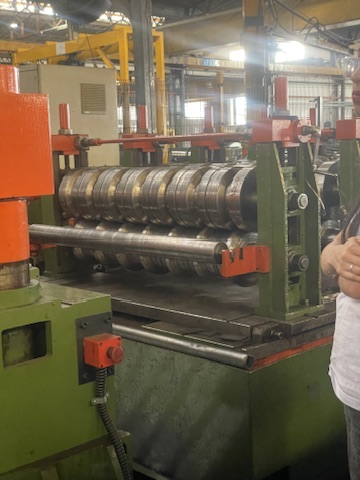
\includegraphics[width=0.75\linewidth]{imagens/slitter-facas-circulares-desbobinamento.jpeg}
  \end{center}
  \fonte{acervo do autor (2026).}
\end{figure}

\subsection{Corte de Precisão (Sistema a Laser)}

O sistema de corte a laser Newton LN 3015F opera com elevada precisão dimensional e permite a programação direta de geometrias complexas via software CAD/CAM. A ausência de ferramental mecânico dedicado significa que o custo de setup para novos formatos é praticamente nulo, pois qualquer geometria contida na área útil da mesa pode ser produzida a partir de um arquivo digital, sem fabricação de punções ou matrizes. Este é o processo adequado para peças com recortes intrincados, furos de posicionamento ou tolerâncias dimensionais críticas. A limitação está na espessura, já que acima de determinado patamar a produtividade cai e o custo sobe em comparação ao plasma.

\subsection{Corte Estrutural (Sistema a Plasma)}

Nos Galpões 4, 5 e 6, o sistema de corte a plasma Oxipira Série Master processa chapas em espessuras entre 0,5 mm e 50 mm, com aplicação predominante em componentes estruturais. Em relação ao laser, o plasma oferece maior produtividade para chapas espessas e menor custo operacional por metro linear nessa faixa, ao custo de tolerância dimensional inferior e rugosidade maior na borda cortada. Para espessuras acima de 15 a 20 mm é frequentemente a única opção economicamente viável entre os processos de corte térmico.

\subsection{Conformação por Dobra (Prensas Dobradeiras)}

As prensas dobradeiras hidráulicas constituem o processo central de conformação do aço na Gravia. O Galpão 1 conta com dez unidades distribuídas entre três modelos: quatro Newton PSH-35030 (comprimento útil de \~{}3 m), seis Newton PSH-7030 (\~{}6 m) e uma hidráulica sincronizada Newton PSH-25030. Os Galpões 4 a 6 abrigam a Newton PSH-55060, com capacidade para peças de até 6 m.

O processo consiste no posicionamento da chapa entre punção e matriz, seguido da aplicação de força hidráulica para produzir a deflexão angular desejada. Parâmetros críticos incluem o raio mínimo de dobra (função da espessura e do limite de resistência do material), o retorno elástico após remoção da carga (springback) que deve ser compensado na programação, e os comprimentos mínimos de flange determinados pelas dimensões do ferramental disponível. Na visita, o que mais chamou atenção nesse setor foi o ruído contínuo das prensas Newton em operação e o volume de peças semi-acabadas empilhadas ao longo do galpão, algo que nenhuma ficha técnica consegue transmitir.

\subsection{Perfilação Contínua (Galpão 3)}

O Galpão 3 opera sob lógica de produção contínua. A perfiladeira recebe a bobina numa extremidade e entrega o perfil acabado pela outra, cortado automaticamente nos comprimentos especificados. O equipamento observado opera a aproximadamente 32 m/min, processa espessuras entre 0,9 mm e 5 mm e trabalha bobinas com largura máxima de 1.200 mm. A tesoura rotativa complementa a linha no processamento contínuo.

\begin{figure}[H]
  \caption{Vista geral da linha de perfilação contínua com tesoura rotativa}
  \label{fig:perfiladeira-linha}
  \begin{center}
    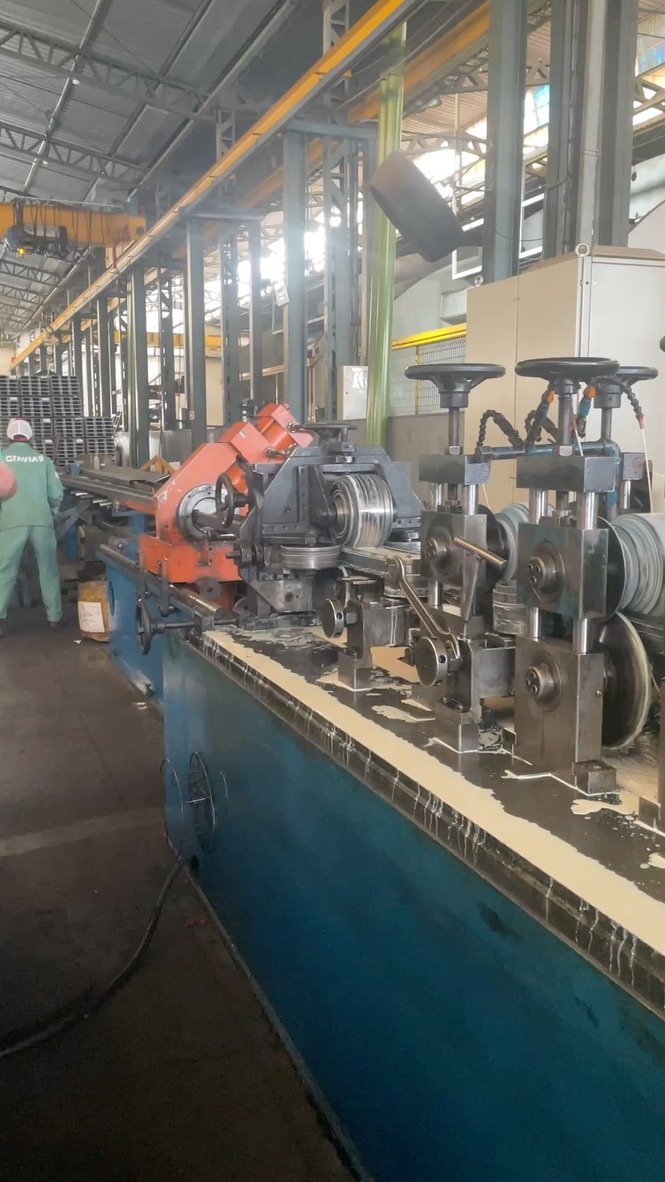
\includegraphics[width=0.85\linewidth]{imagens/perfiladeira-linha-completa-tesoura-rotativa.jpeg}
  \end{center}
  \fonte{acervo do autor (2026).}
\end{figure}

\begin{figure}[H]
  \caption{Chapa de aço em conformação entre rolos da perfiladeira}
  \label{fig:perfiladeira-chapa}
  \begin{center}
    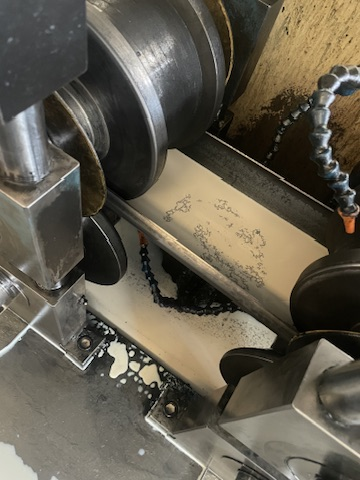
\includegraphics[width=0.75\linewidth]{imagens/perfiladeira-chapa-passando-rolos.jpeg}
  \end{center}
  \fonte{acervo do autor (2026).}
\end{figure}

\begin{figure}[H]
  \caption{Detalhe frontal de estação de rolos conformadores}
  \label{fig:perfiladeira-rolos}
  \begin{center}
    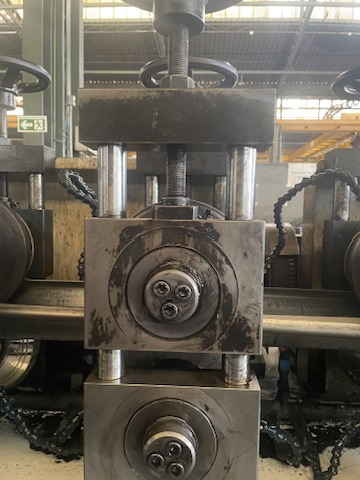
\includegraphics[width=0.75\linewidth]{imagens/perfiladeira-estacao-rolos-frontal.jpeg}
  \end{center}
  \fonte{acervo do autor (2026).}
\end{figure}

Os produtos resultantes (trilhos e montantes para drywall, perfis metálicos, tubos de 2") têm seção transversal constante ao longo de todo o comprimento, característica inerente ao processo de perfilação por rolos.

\begin{figure}[H]
  \caption{Perfis galvanizados para drywall, produto final da perfilação}
  \label{fig:perfis-drywall}
  \begin{center}
    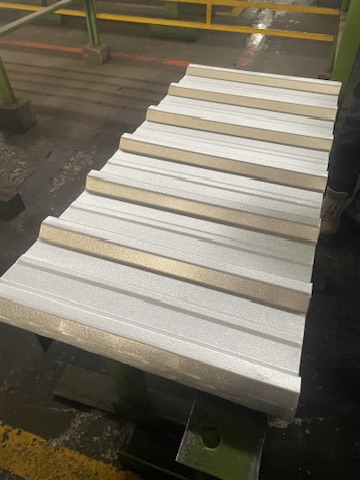
\includegraphics[width=0.75\linewidth]{imagens/perfis-drywall-cortados-empilhados.jpeg}
  \end{center}
  \fonte{acervo do autor (2026).}
\end{figure}

\subsection{Equipamentos Complementares}

A guilhotina hidráulica Newton GHN 301911 atende ao corte reto de chapas de maiores espessuras. A ponte rolante HTB 1787 movimenta chapas e componentes de grande porte ao longo da produção, o que dá a dimensão da escala dos materiais trabalhados. Há também um torno mecânico no Galpão 1, usado para fabricação e manutenção de dispositivos internos. Esse detalhe chama atenção porque indica que a empresa verticaliza parte da sua manutenção em vez de terceirizá-la.

\begin{figure}[H]
  \caption{Ponte rolante HTB 1787 e bobinas de aço ao fundo}
  \label{fig:ponte-rolante}
  \begin{center}
    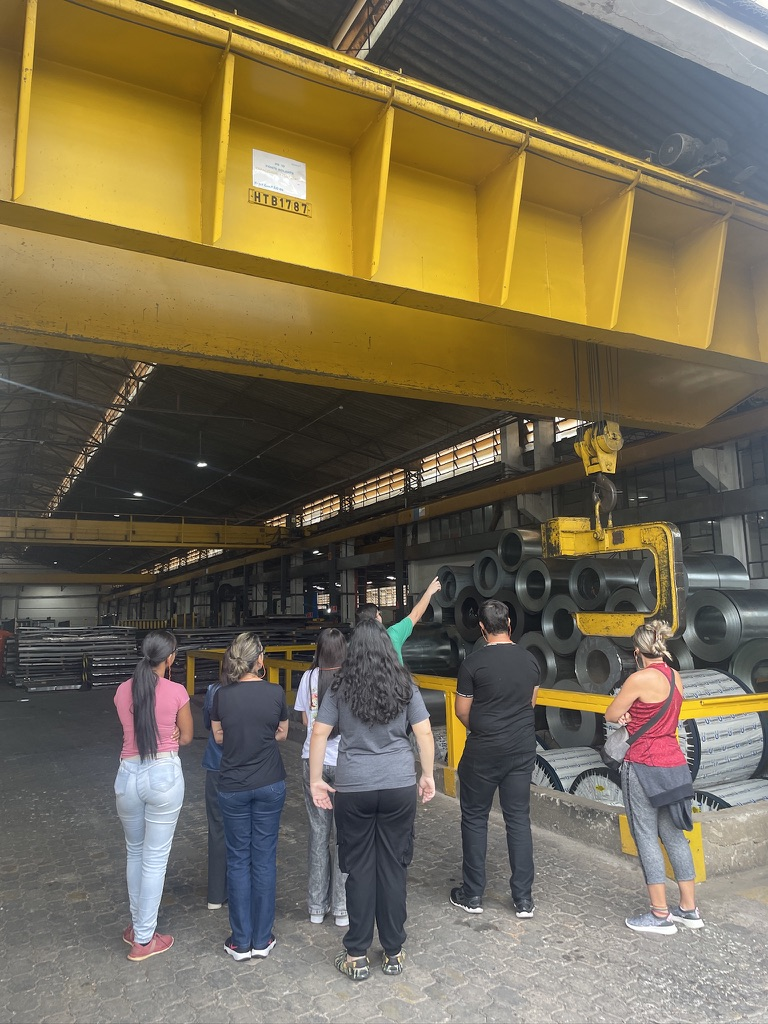
\includegraphics[width=0.85\linewidth]{imagens/ponte-rolante-htb1787-grupo-visitantes.jpeg}
  \end{center}
  \fonte{acervo do autor (2026).}
\end{figure}

\begin{figure}[H]
  \caption{Placa de especificações da guilhotina Newton GHN 3019II}
  \label{fig:guilhotina-placa}
  \begin{center}
    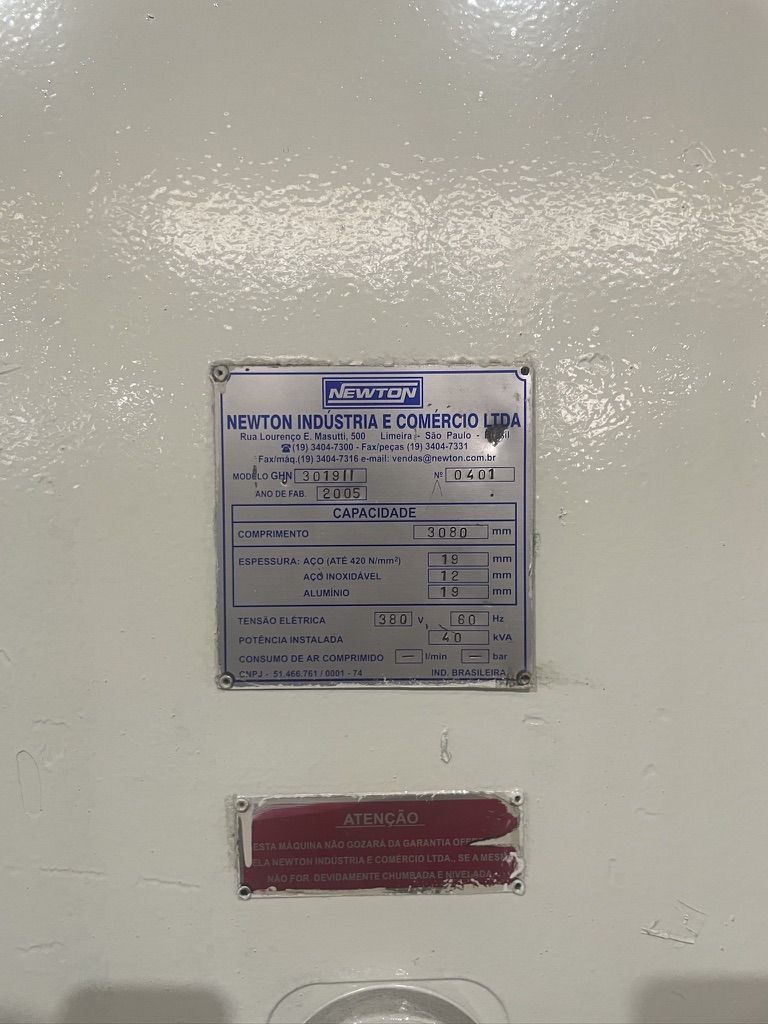
\includegraphics[width=0.6\linewidth]{imagens/placa-guilhotina-newton-ghn3019.jpeg}
  \end{center}
  \fonte{acervo do autor (2026).}
\end{figure}

\section{Quadro-síntese de equipamentos}

\quadrotitle{1}{Equipamentos observados na planta da Gravia}

{\renewcommand{\LTcaptype}{}
\begin{longtable}[]{@{}
  >{\raggedright\arraybackslash}p{(\linewidth - 6\tabcolsep) * \real{0.20}}
  >{\raggedright\arraybackslash}p{(\linewidth - 6\tabcolsep) * \real{0.25}}
  >{\raggedright\arraybackslash}p{(\linewidth - 6\tabcolsep) * \real{0.45}}
  >{\centering\arraybackslash}p{(\linewidth - 6\tabcolsep) * \real{0.10}}@{}}
\toprule\noalign{}
\begin{minipage}[b]{\linewidth}\raggedright
Processo
\end{minipage} & \begin{minipage}[b]{\linewidth}\raggedright
Equipamento
\end{minipage} & \begin{minipage}[b]{\linewidth}\raggedright
Capacidade / Parâmetros
\end{minipage} & \begin{minipage}[b]{\linewidth}\centering
Qtd.
\end{minipage} \\
\midrule\noalign{}
\endhead
\bottomrule\noalign{}
\endlastfoot
Desbobinamento & Desbobinadeira & Alimentação das linhas; conversão bobina $\rightarrow$ chapa & 1 \\
Corte a laser & Newton LN 3015F & Alta precisão; geometrias complexas via software & 1 \\
Guilhotina hidráulica & Newton GHN 3019 & Corte reto; chapas de maiores espessuras & 1 \\
Conformação por dobra & Newton PSH-35030 & Comp. útil \~{}3 m & 4 \\
Conformação por dobra & Newton PSH-7030 & Comp. útil \~{}6 m & 6 \\
Conformação por dobra & Newton PSH-25030 (sinc.) & Dobra de alta precisão & 1 \\
Conformação por dobra & Newton PSH-55060 & Comp. útil até 6 m; componentes estruturais & 1 \\
Torno mecânico & --- & Fabricação interna de dispositivos & 1 \\
Ponte rolante & HTB 1787 & Movimentação de chapas e componentes pesados & 1 \\
Tesoura rotativa & --- & Processamento contínuo de bobinas & 1 \\
Perfilação & Perfiladeira & 32 m/min; larg. máx. 1.200 mm; 0,9--5 mm & 1 \\
Corte a plasma & Oxipira Série Master & 0,5--50 mm de espessura & 1 \\
\end{longtable}
}

\quadrofonte{elaborado pelo autor com base em observação in loco (2026).}

\section{Implicações para o design de produto}

A fabricação em aço não é um processo único, mas uma família de processos com lógicas distintas de custo, precisão e escala. O que a visita à Gravia tornou concreto é que cada escolha projetual sobre o material carrega, embutida, uma escolha sobre como esse material será processado e em que condições econômicas isso se viabiliza.

A escolha entre corte a laser e corte a plasma ilustra bem essa dinâmica. O laser oferece liberdade geométrica com precisão, viabilizando peças com recortes complexos e furos de posicionamento sem ferramental dedicado. O plasma opera com outra lógica, entregando produtividade elevada para chapas espessas ao custo de tolerância dimensional menor. Selecionar entre eles exige considerar espessura do material, tolerância requerida, volume de produção e acabamento superficial. Na prática, um componente estrutural em chapa de 25 mm vai para o plasma, e uma peça de fixação com furo rosqueado de precisão vai para o laser. Foi o que ficou mais evidente na transição entre os galpões durante a visita.

A conformação por dobra, processo central da planta, converte chapas planas em geometrias tridimensionais com custo operacional baixo, desde que o projeto seja compatível com sequências de dobra. Perfis abertos em U, L, Z, C e suas combinações são obtidos com apenas uma operação por dobra. Um projeto que decompõe volumes tridimensionais em séries de operações planares compatíveis com os comprimentos de prensa disponíveis (3 m ou 6 m) é um projeto que a fábrica absorve sem resistência. O conceito de springback merece atenção particular. A chapa tende a recuperar parcialmente sua forma após a remoção da carga, e o programador precisa antecipar esse comportamento antes de executar a primeira dobra. Para o designer, isso significa que ângulos de dobra muito agudos ou tolerâncias angulares muito apertadas exigem compensações que encarecem o processo.

A perfilação contínua opera sob lógica radicalmente diferente. Enquanto as prensas produzem peças discretas, a perfiladeira processa bobinas inteiras em regime contínuo, entregando perfis de seção transversal constante a um custo unitário que nenhum outro processo replica nessa faixa dimensional. Essa eficiência, porém, só se manifesta para seções constantes ao longo do comprimento. Qualquer variação exigiria rolos de geometria variável, com custo e complexidade muito superiores.

A padronização dimensional da planta (chapas de 3 m e 6 m, prensas com comprimentos correspondentes, perfis com bitolas normalizadas) é resultado de décadas de convergência entre capacidades dos equipamentos e demandas do mercado. Para o designer que projeta componentes destinados à construção industrializada, alinhar dimensões do projeto a essas referências reduz custos e aumenta a disponibilidade de fornecedores. Trabalhar com essa gramática em mente permite explorar o que a fábrica pode fazer quando o briefing é suficientemente informado, em vez de simplesmente reproduzir o que ela já faz por inércia.

\section{Conclusão}

A planta da Gravia funciona como um repertório de possibilidades e restrições que o projeto pode explorar ou com as quais precisa negociar. Cada processo observado representa um conjunto específico de liberdades dimensionais, tolerâncias, custos e escalas mínimas de viabilidade.

O que ficou mais claro ao percorrer os galpões foi a lógica de por que cada processo está onde está. A coexistência de laser e plasma no mesmo ambiente produtivo materializa os trade-offs entre precisão e produtividade que permeiam decisões de engenharia de processo. O volume de prensas dobradeiras de diferentes portes mostra que a planta foi configurada em função da diversidade de produtos que precisa atender, e não em torno de uma tecnologia preferencial.

Um designer que conhece o que uma prensa dobradeira de 6 m pode fazer especifica com mais precisão e mais responsabilidade técnica. Sem esse conhecimento, a criatividade projetual frequentemente resulta em peças que não podem ser fabricadas, ou que podem ser fabricadas a um custo que inviabiliza o produto no mercado. A visita à Gravia forneceu esse repertório de forma direta e concreta. O chão de fábrica é mais barulhento, mais sujo e mais revelador do que qualquer capítulo de livro sobre o mesmo assunto.

\section{Referências}\label{referencias}

GRAVIA INDÚSTRIA DE PERFILADOS DE AÇO. Visita técnica à unidade industrial de Taguatinga/DF. [Observação direta]. Taguatinga, DF, 02 jun. 2026.

\end{document}
